\section{Jet Label Definitions}\label{JetLabels}\hfill

Both jets and tracks are characterized by Lorentz 4-vectors $\overrightarrow{J}$ and $\overrightarrow{T}$, respectively. A Lorentz 4-vector is defined as $(E,\overrightarrow{p})$, where E is energy and $\overrightarrow{p}=(p_x,p_y,p_z)$ is the momentum in 3D space. The mass of an object described by a Lorentz 4-vector is defined as $m=\sqrt{E^2-|\overrightarrow{p}|^2}$\footnote{In Natural Units}. Each event, $\mathcal{E}$, is composed of a variable number of jets and each jet is formed by a variable number of associated tracks. Therefore, the fundamental data structure of an event, $\mathcal{E}$, can be interpreted as nested sets. The relationship between jet 4-vector $\overrightarrow{J}$ and the associated track 4-vectors, $\overrightarrow{T}$, is:

\begin{equation}
  \overrightarrow{J}_i = \sum\limits_{j \in \overrightarrow{J}_i} \overrightarrow{T}_{ij}
\end{equation}

While jets get contributions from both hard scatter and pileup, the goal is to recover the hard scatter component. But the actual measured quantities of total energy, $E_{jet}$, and total mass, $m_{jet}$, of each jet contain pileup contamination. To mitigate the effects of pileup, we propose the use of continuous fractions, $E_{frac}$ and $M_{frac}$,\footnote{$E_{frac}$ and $M_{frac}$ can be considered scalar and vector corrections to $\overrightarrow{J}$, respectively. Pileup's stochastic directions affects the vector corrections significantly more than scalar corrections.} to be directly applied to each jet, as ratios, in order to recover only the hard scatter energy, $E_{HS}$, and mass, $m_{HS}$. Therefore, truth labels can be constructed from the 4-vectors of each jet, $\overrightarrow{J}$, by defining:
\begin{equation}
  E_{frac}=\frac{E_{HS}}{E_{jet}} \phantom{.......} M_{frac}=\frac{m_{HS}}{m_{jet}}.
\end{equation}

%As $\left<\mu\right>$ increases from 60 to 200 for the HL-LHC upgrade, the pileup contamination of hard scatter jets will begin to dominate. As PU contamination degrades the quality of HS jets, the task shifts from a binary classification at low pileup conditions to a continuous regression at high pileup conditions. Instead of the traditional binary labels as HS or PU, 
%We introduce a continuous labels for Energy and Mass Fraction, Efrac and Mfrac, which represents the fraction of the jets energy and mass originating from pileup. To construct these continuous labels, we sum over the Lorentz Four-Vector of the tracks, $\overrightarrow{T_i} = (E,p_x,p_y,p_z)_i = (E,\overrightarrow{p})_i = (T_0, T_1, T_2, T_3)_i$, which are truth-associated to each jet, $\overrightarrow{J}$:

%\begin{equation}
%    \overrightarrow{J}_{HS} = \sum\limits_{i \in \text{HS}} \overrightarrow{T}_i \phantom{............} \overrightarrow{J}_{PU} = \sum\limits_{i \in \text{PU}} \overrightarrow{T}_i \\
%    %\overrightarrow{J}_{Total} = \overrightarrow{J}_{HS} + \overrightarrow{J}_{PU} 
%\end{equation}

%Now that we have the four vector HS and PU contributions of each jet, we can directly evaluate the Energy and Mass fractions on a per jet basis. The total Lorentz Four-Vector is simply the sum of the HS and PU contributions, $\overrightarrow{J}_{Total} = \overrightarrow{J}_{HS} + \overrightarrow{J}_{PU}$. Note that Energy is the first component of the jets Four-Vector, $J_0=E$, and mass is found using the relativistic energy relations in natural units, $m^2=E^2-|\overrightarrow{p}|^2$. These expressions can be used to derive the labels used for regression.

%\begin{equation}   
%    Efrac = \frac{E_{HS}}{E_{Total}} \phantom{............} Mfrac = \frac{m_{HS}}{m_{Total}}
%\end{equation}


%\begin{figure}[ht]
%\centering
%\begin{subfigure}{.5\textwidth}
% \centering
%  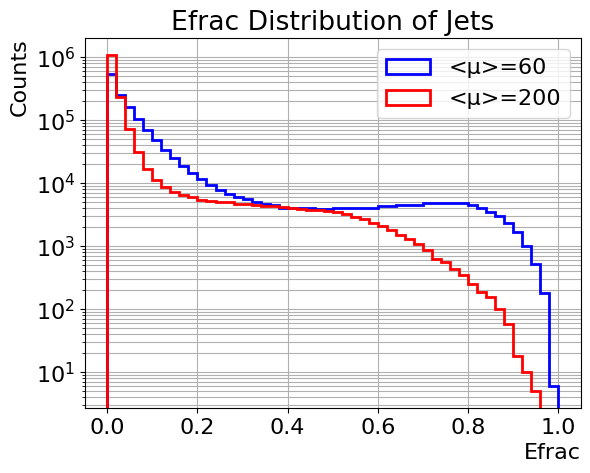
\includegraphics[width=1\linewidth]{Efrac}
%  \caption{}
%  \label{fig:sub1}
%\end{subfigure}%
%\begin{subfigure}{.5\textwidth}
%  \centering
%  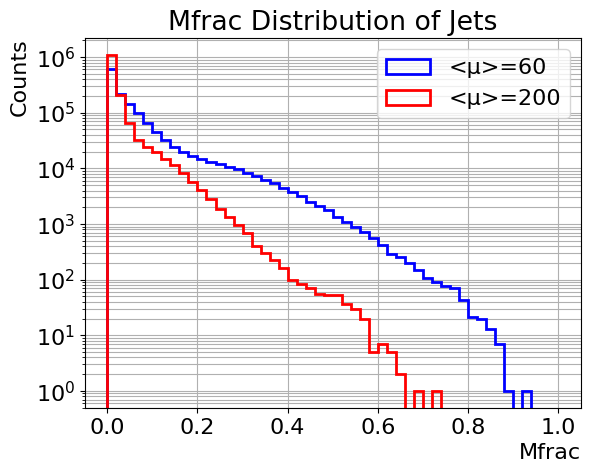
\includegraphics[width=1\linewidth]{Mfrac}
%  \caption{}
%  \label{fig:sub2}
%\end{subfigure}
%\caption{The truth energy and mass fractions used for the continuous regression task at $\left< %\mu \right> = 60$ and $\left< \mu \right> = 200$. These fractions can be applied to jets to %recover the hard scatter contributions.}
%\label{fig:Labels}
%\end{figure}

%The pileup mitigation problem can be formulated in two ways: a binary classification problem where a jet is considered hard scatter if a significant fraction of its energy and mass originate from hard scatter tracks or as a regression problem where the model directly predicts energy and mass fractions from pileup tracks. As $\left\langle \mu \right\rangle$ increases, the pileup contamination becomes so large that all jets begin to have significant contribution to their mass and energy from pileup tracks. By promoting the binary classification problem to a regression problem through continuous energy and mass fraction labels, allows for useful and physically significant jet characteristics independent of $\left\langle \mu \right\rangle$. 

%\arun{How does introducing continuous energy and mass fraction helps mitigating pileup? This motivation is required to make our work unique.}

For the first time, this article proposes to simplify the pileup mitigation strategy by directly applying $E_{frac}$ and $M_{frac}$ labels to simultaneously identify pileup and apply corrections to hard scatter jets through the use of attention neural networks. This approach uses all available information from an event, including the correlations manifesting in hard scatter processes, to get a more accurate representation of the underlying physics process. Using a simulated dataset, the proposed approach outperforms traditional pileup mitigation strategies and assists with physics analysis.


%\luke{1) This is the first time we use continuous labels to characterize pileup. 2) The underlying physics HS processes often results in correlated jet sets (same for dijet PU) and we are using the labels to recover the mass and energy of underlying physics processes. 3) The novelty of this approach is we provide calibration of jets to provide a more accurate picture of the event. Simultaneous identification and energy and mass calibration. And full scale analysis using 100\% of information.}

%Through the use of attention and transformer encoder stacks, the hard scatter structure of a jet can be recovered and the stochastic pileup background can be suppressed.
